\chapter{Introduction}


\label{chapter:introduction}


\section{Proposal Summary}

The aim of this project is to build a domain specific question answering engine to provide mothers, and prospective mothers with answers to breastfeeding related queries. The final product should accept natural language questions from users and, where possible, retrieve relevant answers. When those answers are not available in the knowledge base, the user should be not provided an inaccurate answer, but rather given a message detailing that the question was not automatically answerable, or the question should be escalated to a healthcare professional that can address it.


\section{Rationale}

While machine learning has seen significant and sustained increase in usage in healthcare most of that research has mainly focused on Imaging, Public Health and Bioinformatics \cite{7801947}. Patient facing question answering systems and chatbots have seen widespread usage \cite{doi/10.2196/18301}, seeing significant success in the mental health space \cite{doi/10.2196/jmir.7023}. Conversational agents have been built for the specific purpose of assisting mothers in regard to breastfeeding, with Public Heath England, through the Start4Life Breastfeeding Friend chatbot, found that new mothers reported they were more likely to attempt breastfeeding than not (59\%, n=1000), when in conjunction with other support strategies \cite{phe.start4life}. Given the success rate of the Start4Life initiative, which provides answers to 42 pre-defined questions \cite{start4life.faq}, a more novel approach using information retrieval techniques should lead to a higher number of possible questions receiving successful answers.

\section{Personal Motivation}

I have been working in Machine Learning for the last five years, with a heavy focus on NLP. I have been able to work on a wide breadth of problems during my career, but while being very interested in the subject, I have never had an opportunity to commercially implement a question and answer system. At the same time, most of my work has had a strictly commercial focus, so being able to work towards a project with a positive social impact is something that drove me to select this specific topic.

\section{Objectives}

The primary objective of the project is to produce accurate answers to breastfeeding related questions. This can be further refined into 3 secondary objectives:
\begin{itemize}
	\item \textbf{Identifying the question type}: Questions must first be divided between factoid questions, and questions containing context.
	\item \textbf{Retrieving the relevant passage for questions}: Extract the passages that may be potential answers for the question, and rank them by relevance.
	\item \textbf{Extracting the specific factoid from the passage}: Find the specific answer to the question within a passage, extracting the relevant keywords or sentence chunks.
\end{itemize}


\section{Hypothesis}
It is the aim of the project to prove that, given a set of training questions and answers, as well as a tagged of expert articles, user breastfeeding related user generated questions can be answered accurately.


\section{Methodology}
The main data source for the project is the platform \href{https://lactapp.com/}{LactApp}. Two separate sources from the application will be used:
\begin{itemize}
	\item \textbf{Expert content}: The platform contains numerous expert written articles regarding most aspects related to breastfeeding, categorized by topic and other classifications.
	\item \textbf{Conversations}: The live chat functionality has collected conversations between mothers and experts. These range from general factual questions (e.g. "How often do newborns feed?"),
	 to very specific questions requiring contents (e.g. "I suspect my 3-month-old has bronchitis and is not latching, what should I do?").
\end{itemize}
As well as these two datasets other breastfeeding FAQ documents and sites will be used to train the restricted domain model.

\subsection{Research Strategy}
The initial stage of the project will consist of evaluating the current state of the art in terms of research. This will be focused on the four main paradigms of question answering \cite{CALIJORNESOARES2020635}: Natural language processing and understanding, information retrieval, knowledge base retrieval, and hybrid methods, with a focus on restricted domain question answering. As part of the literature review, current technology implementations will also be evaluated, including, but not limited to, BERT \cite{devlin2018bert}, Haystack \cite{haystack.whatis} as well as other information retrieval systems.

The second stage of the project will focus on evaluating the datasets and separating the training and testing datasets. The data cleaning strategy will also be defined and implemented at this stage. Once the data has been prepared, and a testing dataset defined, the representative sample of questions will be set aside for evaluating the model at the conclusion of the project.

The third stage will consist of building the question answering model iteratively, testing the improvement in quality with each modification applied to the pipeline, including features generated, tweaking machine learning models, or adding new stages on the pipeline.


\subsection{Project Methodology}
The desired outcome of the project is to create a new product, by adapting existing open source tools, training custom models for the target data, and using commercially available tools to build an end-to-end solution that can assist mothers with their breastfeeding queries, served via an API.

\subsection{Project Plan}
As detailed in figure \ref{fig:gantt}, the project plan has been scheduled finish the implementation work by the 25th of December, and the finished paper by the 8th of January.

\begin{figure}[h]
	\caption{Project Gantt Chart}
	\centering
	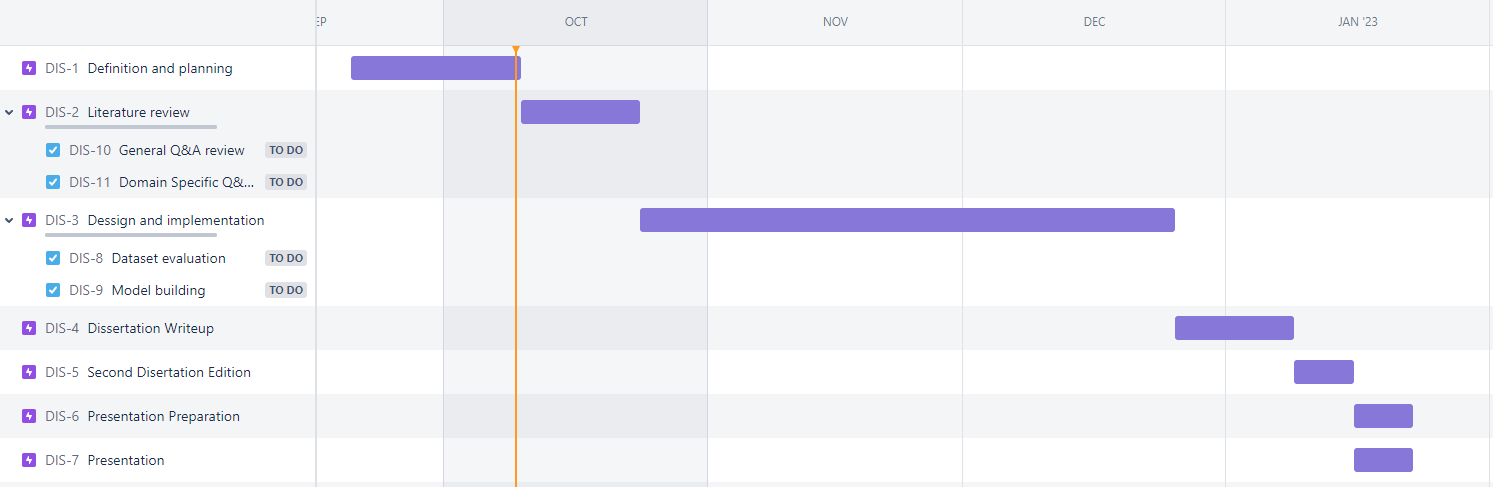
\includegraphics[width=16cm]{plan.png}
	\label{fig:gantt}
\end{figure}

\section{Global ethical commitment and Sustainable Development Objectives}
If the question answering accuracy is high enough, the project should reduce the turn-around time for mothers' queries, leading to better advice access for end users.
\subsection{Sustainability}
The main carbon footprint impact of the project will likely be in compute, given the size of the dataset, the likelihood is that the impact on the environment will be minor, given that the bulk of the work will be performed on a single, consumer grade hardware, workstation.
\subsection{Diversity and Inclusivity}
Active care will be taken to ensure that any biases present in the training data do not carry to the machine learning model. A more specific strategy will be devised after evaluating the training dataset.
\subsection{Ethical behaviour and social responsibility}
The data used will be anonymized and kept secure, limiting both the likelihood of data leaks, as well as mitigating the potential impact on the platform users. 